%\documentclass[10pt, a4paper]{article}
\documentclass[submit]{smj}

\usepackage[utf8]{inputenc}
\usepackage{amsmath, amssymb, amsthm, bbm}
\usepackage{xcolor}
\usepackage{graphicx}
\usepackage[authoryear]{natbib}
\usepackage{apalike}
\usepackage{relsize}
\usepackage{array}
\usepackage{multirow}
%\usepackage{showlabels}
\usepackage{setspace}
\usepackage[normalem]{ulem}
\usepackage{xspace}
%Add line numbering
%Line numbering can be incorporated by using the lineno package. Add these statements in the preamble:
%\usepackage{lineno}
%\linenumbers

%\usepackage[nomarkers,figuresonly]{endfloat}

\DeclareMathOperator*{\argmax}{arg\,max}

\newtheorem{prob}{Problem}
\newtheorem{prop}{Proposition}
\newtheorem{definition}{Definition}
\theoremstyle{definition}
\newtheorem{defn}{Definition}[section]
%%%%% bold symbol in math enviornment
\newcommand{\m}[1]{\boldsymbol{#1}}

\newcommand{\fmm}{\textsc{fmm}\xspace}
\newcommand{\X}{\text{\textbf{X}}}
\newcommand{\pkg}[1]{{\fontseries{b}\selectfont #1}} 

\Title{Merging the components of a finite mixture using  posterior probabilities}
\TitleRunning{Merging the components of \fmm}
\Author{Marc Comas-Cufí\Affil{1}, Josep A. Martín-Fernández\Affil{1}, Glòria Mateu-Figueras\Affil{1}}
\AuthorRunning{Marc Comas-Cufí \textrm{et al.}}

\Affiliations{
\item Department of Computer Sciences, Applied Mathematics and Statistics, 
      Polytechnic School, 
      University of Girona,
      Spain
}

\CorrAddress{Josep A. Martín-Fernández, Department of Computer Science, Applied Mathematics and Statistics,
      University of Girona, P-IV, Campus Montilivi, E-17071 Girona, Spain}
\CorrEmail{josepantoni.martin@udg.edu}
\CorrPhone{(+34)\;972\; 418\;426}
\CorrFax{(+34)\;972\;418\;792}

\Abstract{
Methods in parametric cluster analysis commonly assume that data can be modelled by means of a finite mixture of distributions. Different authors show that associating each mixture component to one cluster is frequently misleading because different mixture components overlap forming a unique cluster. A generic approach to build a hierarchy of mixture components generalises the most important techniques earlier proposed in the literature. Using the information provided by the posterior probabilities the iterative merging process constructs the clusters. This generic approach also permits to define other merging indices. A new approach based in the log-ratio of posterior probabilities is introduced. Simulated and real datasets are used to illustrate its performance.
}

\Keywords{
Model-based clustering; Mixture model; Hierarchical clustering; Merging components; Log-ratio; Simplex
}
\begin{document}

%\begin{spacing}{1.9}
%%%%%%% BEGIN SPACING


\pagenumbering{arabic}

\maketitle

\section{Introduction}


% Mixture models
A common approach in parametric cluster analysis assumes data can be modelled by means of a \emph{finite mixture of distributions} \citep{fraley2002model, punzo2014flexible}, also called \emph{finite mixture model} (\fmm). A \fmm is a probability distribution whose probability density function (pdf) is a linear combination of different distributions with same domain $\mathbb{X}$. More precisely, the pdf $f$ of a \fmm is
\begin{equation}\label{mixt}
f(\;\cdot\; ; \pi_1, \dots, \pi_k, \m\Theta) = \pi_1 f_1(\;\cdot\; ; \m\theta_1) + \dots + \pi_k f_k(\;\cdot\; ; \m\theta_k),
\end{equation}
where $\m\Theta =\{ \m\theta_1, \dots, \m\theta_k\}$, $\m\theta_j$ are the parameters of pdf $f_j$, $1\leq j \leq k$, and $\pi_j$ is the ``weight'' of component $f_j$. Restriction $\sum_{\ell = 1}^k \pi_\ell = 1$ guarantees that  $\int_{\mathbb{X}}f = 1$. Originally, the clustering algorithm based on a \fmm follows two steps:
\begin{enumerate}
\item using the information provided by a sample $\X=\{\m x_1, \dots, \m x_n\}$, to calculate estimates $\hat{\pi}_1, \dots, \hat{\pi}_k$ and $\hat{\m\Theta}$ of parameters $\pi_1, \dots, \pi_k$ and $\m\Theta$, and
\item to classify each observation $\m x_i \in \X$ according to the criterium of maximizing the posterior probability
\[
\tau_{ij}= \frac{ \hat{\pi}_j f_j(\m x_i ; \hat{\m\theta}_j) }{\sum_{\ell=1}^k \hat{\pi}_\ell f_\ell(\m x_i ; \hat{\m\theta}_\ell) },
\]
that is, one observation $\m x_i$ is classified to cluster $c$ if
\begin{equation}\label{map_criteria}
c = \argmax_{j=1}^k \tau_{ij}.
\end{equation}
\end{enumerate}
Note that in this process, the number of clusters $k$ is equal to the number of mixture components. \cite{mclachlan2014components} presents a recent review of different approaches used to decide the value of $k$. From the reviewed approaches, we use the Bayesian Information Criterion (BIC) to fit the number of mixture components. The use of BIC to decide the number of components is justified by \cite{keribin1998consistent, keribin2000consistent}, who shows that under certain regularity conditions it estimates the number of mixture components consistently. \cite{fraley1998how} show that the BIC is effective as a model selection criteria  at practical level.

On the other hand, \cite{lee2004combining}, \cite{hennig2010methods}, \cite{baudry2010combining}, \cite{melnykov2013distribution} and \cite{pastore2013merging} propose to separate the concepts of cluster and mixture component. The authors show that associating each mixture component to one cluster can be misleading because frequently different mixture components are so overlapped that they can be considered as a unique cluster. In other words, one cluster could be formed by the result of merging two different mixture components. According to this approach, the \fmm clustering algorithm is completed with a third step:

\begin{itemize}
\item[3.] to analyse which of the $k$ mixture components should be merged to form $k'$ clusters, $k' \leq k$.
\end{itemize}

The crucial point of this new step is how to decide which components have to be merged. Note that considering different components as a single cluster do not change the underlying finite mixture, therefore for a given sample the likelihood is not modified. This makes impossible to decide which components form a single clusters in terms of the likelihood or through the BIC criteria \citep{hennig2010methods}. The approaches presented in this paper are based on the posterior probabilities which are obtained after adjusting a \fmm. In this article we introduce a generic approach that generalises methods given by \cite{baudry2010combining}, \cite{hennig2010methods} and \cite{longford2014}. With this new approach, the analyst can define its own criteria, for example, a criteria based in log-ratio transformations of posterior probabilities \citep{aitchison1986statistical}. Using this generic approach for merging components one can build a hierarchy over the set of mixture components. From this hierarchical structure, the analyst can decide the final clustering.

The paper is organised as follows: in Section~\ref{definitions} some definitions and notations used throughout this paper are introduced. In Section~\ref{generic_merging} the generic merging approach is presented. It is shown how most important criteria from literature reduce to this generic approach. Using the generic merging approach, Section~\ref{logratio_section} presents a new family of criteria based on the log-ratio approach. In Section~\ref{merging_examples_dist}, we present two examples to illustrate the algorithm with different types of mixture distributions. To conclude, final remarks are given in Section~\ref{remarks}.

\section{Definitions and notation}\label{definitions}

%
Let $\mathcal{I}^k = \{1, \dots, k\}$ be a set of natural numbers to indicate the components of a \fmm. A \emph{partition} of $\mathcal{I}^k$ of size $s$, $\mathcal{P}_s$, is the disjoint union of subsets $I_p$, called \emph{parts}. More formally, $\mathcal{P}_s$ is a set with $s$ subsets $I_p$  that $\bigcup_{I_p \in \mathcal{P}_s} I_p = \mathcal{I}^k$ and for any two parts $I_a, I_b \in \mathcal{P}_s$ with $a \neq b$, $I_a \cap I_b = \emptyset$ holds. Given a partition  $\mathcal{P}_s$, the pdf $f$ of a \fmm (Equation~\ref{mixt}) can be rewritten as
\begin{equation}
f = \pi_{I_1} f_{I_1}(\;\cdot\;; \m\Theta) + \dots + \pi_{I_s} f_{I_s}(\;\cdot\;; \m\Theta),
\label{mixt_part}
\end{equation}
where $f_{I_p}(\;\cdot\;;  \m\Theta) = \sum_{j \in I_p} \frac{\pi_j}{\pi_{I_p}} f_j(\;\cdot\; ; \m\theta_j)$ and $\pi_{I_p} = \sum_{\ell \in I_p} \pi_\ell$. Note that using this notation each $f_{I_p}(\;\cdot\;;  \m\Theta)$ is also a \fmm. Because each part $I_p$ defines a single component $f_{I_p}$, where there is no confusion, we use $I_p$ referring either to the part $I_p$ or to the component $f_{I_p}$. Note that, given $k$ components of a \fmm $f$, there is $B_k$ different ways to express the mixture  $f$ in terms of a partition.\footnote{$B_k$ is the $k$-th Bell number defined recursively as $B_0 = 1$ and $B_k = \sum_{i=0}^{k-1} \binom ni B_{i-1}$.}



A \emph{hierarchical sequence of partitions of $\mathcal{I}^k$} is a sequence $\mathcal{P}_1, \dots, \mathcal{P}_k$ verifying that
\begin{itemize}
\item $\mathcal{P}_1$ is the one-part partition $\mathcal{P}_1 = \{ \mathcal{I}^k \}$,
\item if a part $I_p \in \mathcal{P}_{s-1}$ then either there is a part $I_a \in \mathcal{P}_{s}$ with $I_p = I_a$ or there are two parts $I_a, I_b \in \mathcal{P}_s$ with $I_p = I_a \cup I_b$, and
\item $\mathcal{P}_k= \{ \{1\},\{2\}, \dots, \{k\} \}$.
\end{itemize}



One can extend Equation~\ref{map_criteria} in terms of partitions. Indeed, let $\X = \{\m x_1,\dots, \m x_n\}$ be a sample formed by observations of $\mathbb{X}$. Given a partition $\mathcal{P}_s = \{ I_1, \dots, I_s \}$, we define the posterior probability of $\m x_i$ being classified to part $I_p\in \mathcal{P}_{s}$ as
\[
\tau_{i I_p} =  \frac{ \hat{\pi}_{I_p} f_{I_p}(\m x_i; \hat{\m\Theta}) }{\sum_{\ell=1}^s \hat{\pi}_{I_\ell} f_{I_\ell}(\m x_i; \hat{\m\Theta})}
\]
where $\hat{\pi}_{I_p} = \sum_{\ell \in I_p} \hat{\pi}_\ell$.

For the partition  $\mathcal{P}_s$, we define the posterior probability vector associated to observation $\m x_i$ as
\begin{equation}\label{ppv}
\m\tau_{i \mathcal{P}_s} = \left(\tau_{i I_1} , \dots, \tau_{i I_s}  \right).
\end{equation}
The posterior probability vector $\m \tau_{i \mathcal{P}_s}$ denotes the conditional probability that $\m x_i$ arises from mixture components $f_{I_1}, \dots, f_{I_s}$. Since $\mathcal{P}_s$ is a partition $\sum_{p=1}^s \tau_{i I_p} = 1$ holds  for $1 \leq i \leq n$. Similarly to Equation~\ref{map_criteria}, the posterior probability vectors $\m\tau_{i \mathcal{P}_s}$ can be used to classify $\m x_i \in \X$ to the cluster $c$ if
\begin{equation}\label{cluster_criteria}
c= \argmax_{p=1}^s \{ \tau_{i I_p} \}.
\end{equation}

Let $\text{\textbf{T}}_{\mathcal{P}_s}$ be the matrix with $n$ rows and $s$ columns formed by the $n$ vectors of posterior probabilities $\m \tau_{i\mathcal{P}_s}$ associated to partition $\mathcal{P}_s$. For example, $\text{\textbf{T}}_{\mathcal{P}_k}$ is the initial matrix, when the number of components and clusters are equal. Importantly, by Equation \ref{ppv}, any matrix $\text{\textbf{T}}_{\mathcal{P}_s}$ can be obtained from matrix $\text{\textbf{T}}_{\mathcal{P}_k}$ respectively aggregating the corresponding columns of parts $I_1, \dots, I_s$.


\section{Generic approach}\label{generic_merging}

\subsection{General merging criteria}\label{merging_criteria}

Let $\text{\textbf{X}} = \{\m x_1,\dots,\m x_n \}$ be a sample defined in  a domain $\mathbb{X}$ and let $f$ be a \fmm with $k$ components defined on $\mathbb{X}$ (Equation~\ref{mixt}). Given a partition $\mathcal{P}_s = \{I_1, \dots, I_s\}$, let $\m\tau_{i \mathcal{P}_s}= \left( \tau_{i I_1} , \dots, \tau_{i I_s}  \right)$ be the posterior probability vector associated to observation $\m x_i$ for $i$, $1\leq i \leq n $.

For a partition $\mathcal{P}_s$  and matrix of posterior probabilities $\text{\textbf{T}}_{\mathcal{P}_s}$ we propose to merge those two parts $I_a, I_b \in \mathcal{P}_s$ maximising the weighted mean
\begin{equation}\label{unifying_equation}
S_{\omega, \lambda}( \text{\textbf{T}}_{\mathcal{P}_s},  I_a,  I_b) = \frac{\sum_{i=1}^n \omega(\m\tau_{i \mathcal{P}_s}, I_a, I_b) \; \lambda(\m\tau_{i \mathcal{P}_s}, I_a, I_b)}{\sum_{i=1}^n \omega(\m\tau_{i \mathcal{P}_s}, I_a, I_b) }.
\end{equation}
where $\omega(\m\tau_{i \mathcal{P}_s}, I_a, I_b)$ is a non-negative function and $\lambda(\m\tau_{i \mathcal{P}_s}, I_a, I_b)$ is a function measuring the preferences for the researcher in merging components $I_a$ and $I_b$. Function $\omega(\m\tau_{i \mathcal{P}_s},  I_a,  I_b)$ is a weigh function. It permits to modify the influence each posterior probability vector $\m\tau_{i \mathcal{P}_s}$ has to calculate Equation~\ref{unifying_equation} for parts $I_a$ and $I_b$, we call the value of Equation~\ref{unifying_equation} \emph{the $S$-value from $I_a$ to $I_b$}. Function $\lambda(\m\tau_{i \mathcal{P}_s},  I_a,  I_b)$ is an utility function. It measures our preferences to consider components $f_{I_a}$ and $f_{I_b}$ as a single component, and therefore, to model a single cluster by means of the merged component $f_{I_a \cup I_b}$.


Starting from partition $\mathcal{P}_k = \{ \{1\}, \dots, \{k\} \}$, where the number of clusters is equal to the number of components, two parts are merged according to the maximum of Equation~\ref{unifying_equation}. Iteratively repeating this process until partition $\mathcal{P}_1$ is obtained, the algorithm builds an agglomerative hierarchical sequence of partitions. Remarkably, by the definition of functions $\omega$ and $\lambda$, the process only depends on the posterior probability vectors $\text{\textbf{T}}_{\mathcal{P}_s}$. Indeed, the behaviour of function $S$ is completely determined by the choice of function $\omega$ and $\lambda$.

For any partition $\mathcal{P}_k$ we need to calculate $k^2-k$ different $S$-values to identify the maximum. The process is repeated for partition $\mathcal{P}_{k-1}$ until $\mathcal{P}_1$, calculating a maximum of $\frac{k^3-k}{3}$ $S$-values. This quantities are reduced by half when functions $S_{\omega, \lambda}$ is symmetric. 

\subsection{Minimising the final entropy}
\label{entropy_section}

\cite{baudry2010combining} propose an algorithm to build a hierarchical sequence of partitions based on the concept of entropy. The Shannon entropy of a posterior probability vector $\m\tau_{i \mathcal{I}_s} = \left( \tau_{i I_1} , \dots, \tau_{i I_s}  \right)$ is
\[
\text{Ent}( \m\tau_{i \mathcal{P}_s} ) = -\sum_{j=1}^s \tau_{i I_j}  \log(\tau_{i I_j} ).
\]

The entropy can be interpreted as a measure of similarity between a probability vector and the probability vector $\m\tau^0_{s}=\left(\frac{1}{s}, \dots, \frac{1}{s}\right)$, taking the maximum value when $\text{Ent}\left( \m\tau^0_{s} \right) = log(s)$. Given partition $\mathcal{P}_s = \{ I_1, \dots, I_s\}$ the algorithm iteratively merges  the two mixture components optimising the overall entropy. Let $\mathcal{P}_{s-1}^{I_a\cup I_b}$ be the partition obtained after merging components $I_a$ and $I_b$ from $\mathcal{P}_s$. The parts $I_a$ and $I_b$ merged minimise expression
\[
\sum_{i=1}^n \text{Ent}( \m\tau_{i \mathcal{P}_{s-1}^{I_a\cup I_b}} ).
\]

According to \cite{baudry2010combining}, minimising previous expression is equivalent to maximise the loss of entropy, that is, to maximise the sum of differences
\[
\sum_{i=1}^n  \left\{ \text{Ent}( \m\tau_{i \mathcal{P}_s} ) - \text{Ent}( \m\tau_{i \mathcal{P}_{s-1}^{I_a\cup I_b}} ) \right\}.
\]
which can be written only in terms of $\tau_{i I_a}$  and $\tau_{i I_b}$ as
\begin{equation}\label{entropy}
\sum_{i=1}^n   \left\{(\tau_{iI_a}+\tau_{iI_b}) \log(\tau_{iI_a} + \tau_{iI_b}) - \left[\tau_{iI_a} \log(\tau_{iI_a}) + \tau_{iI_b} \log(\tau_{iI_b})\right] \right\}.
\end{equation}
We define function $\lambda_{\,\Delta\text{Ent}}$ as
\[
\lambda_{\,\Delta\text{Ent}}(\m\tau_{i \mathcal{P}_s},  I_a,  I_b) :=  (\tau_{iI_a}+\tau_{iI_b}) \log(\tau_{iI_a} + \tau_{iI_b}) - \left[ \tau_{iI_a} \log(\tau_{iI_a}) + \tau_{iI_b} \log(\tau_{iI_b}) \right],
\]
and function $\omega_{\text{cnst}}$ constant, for example 
\[
\omega_{\text{cnst}}(\m\tau_{i \mathcal{P}_s},  I_a,  I_b) := 1.
\]

In this approach, because $\omega_{\text{cnst}}$ is constant,  we are considering each observation equally important to compute the $S$-value. The weighing is independent of parts $I_a$ and $I_b$ we are willing to merge. In this case, the $S$-values (Equation~\ref{unifying_equation}) take the form
\[
\begin{split}
S_{\text{cnst}, \Delta\text{Ent}}( \text{\textbf{T}}_{\mathcal{P}_s},  I_a,  I_b) = \frac{1}{n} \sum_{i=1}^n & \left\{(\tau_{iI_a}+\tau_{iI_b}) \log(\tau_{iI_a} + \tau_{iI_b}) - \right.\\ 
&\quad \left.\left[ \tau_{iI_a} \log(\tau_{iI_a}) + \tau_{iI_b} \log(\tau_{iI_b}) \right]\right\}.
\end{split}
\]

Note that in this approach function $S_{\text{cnst}, \Delta\text{Ent}}$ is symmetric with respect $I_a$ and $I_b$. Therefore, for partition $\mathcal{P}_k$ we only need to calculate $\frac{k^2-k}{2}$ $S$-values. Note also that for partition $\mathcal{P}_{k-1}$ we only need to update the value of $k-2$ $S$-values. To complete the process of merging we only need to calculate $(k-1)^2$ different $S$-values. 

%$\frac{k^2-k}{2} + \sum_{\ell=1}^{k-2} \ell$

\subsection{Maximising the misclassification probability}
\label{missclassification_section}

\cite{hennig2010methods} proposes to merge the components $I_a$ and $I_b$ from $ \mathcal{P}_s$ that maximise \emph{the probability of classifying to component $I_b$ an observation generated from component $f_{I_a}$ }. To estimate this probability,  \cite{hennig2010methods} introduces a consistent estimator, the Directed Estimated Misclassification Probabilities (DEMP) defined as
\[
\frac{ \frac{1}{n} \sum_{i=1}^n {\tau_{iI_a} \mathbbm{1}\left( \forall j\; \tau_{i I_{b}} \geq \tau_{iI_j} \right)}}{ \hat{\pi}_{I_a}},
\]
where $\mathbbm{1}\left( \cdot \right)$ is the indicator function. Because $ \hat{\pi}_{I_a} = \frac{1}{n} \sum_{i=1}^n \tau_{iI_a}$, the estimator DEMP can be written in terms of posterior probability as
\begin{equation}\label{demp_criteria}
\frac{ \sum_{i=1}^n {\tau_{iI_a} \mathbbm{1}\left( \forall j\; \tau_{i I_{b}} \geq \tau_{iI_j} \right)}}{\sum_{i=1}^n \tau_{iI_a} }.
\end{equation}

Note that when parts parts $I_a$ and $I_b$  overlaps, Equation~\ref{demp_criteria} take higher values because many observations generated by $I_a$ takes a largest posterior probability $\tau_b$.

In consequence, the estimator DEMP (Equation~\ref{demp_criteria}) is equivalent to set $\omega :=\omega_{\text{cnst}}$ and  $\lambda := \lambda_{\text{DEMP}}$ where
\begin{equation}\label{lambda_demp}
\lambda_{\text{DEMP}}(\m\tau_{i \mathcal{P}_s},  I_a,  I_b) := \mathbbm{1}\left( \forall j\; \tau_{i I_{b}} \geq \tau_{iI_j} \right)
\end{equation}
and
\[
\omega_{\text{prop}}(\m\tau_{i \mathcal{P}_s},  I_a,  I_b) :=  \tau_{iI_a}.
\]

In this approach function $\lambda_{\text{DEMP}}$ is giving preference to those observations $x_i$ classified to part $I_b$. Moreover, $\omega_{\text{prop}}$ function is weighing higher those observations with high posterior probability $\tau_{iI_a}$. This approach permits to calculate the $S$-value from $I_a$ to $I_b$ measuring our preference to merge $I_a$ into $I_b$. Note that in this case function  $S_{\,\text{DEMP}}$ is not symmetric, therefore, in this case the total number of $S$-values needed to complete the process is $2 (k-1)^2$.

A variation of \cite{hennig2010methods} approach is proposed by \cite{longford2014}. Instead of considering function $\lambda_{\text{DEMP}}$ given by Equation~\ref{lambda_demp}, in this case the preference for merging $I_a$ into $I_b$ is given by
\[
\lambda_{\text{DEMP}_m}(\m\tau_{i \mathcal{P}_s},  I_a,  I_b) = \frac{\tau_{iI_b}}{\tau_{iI_a} + \tau_{iI_b}}.
\] 
Function $\lambda_{\text{DEMP}_m}$, similarly to function $\lambda_{\text{DEMP}}$, is giving higher score to those observations with higher posterior probability, $\tau_{iI_b}$, of being generated by component $f_{I_b}$ conditioned to those observations being generated either by $f_{I_a}$ or $f_{I_b}$.


\section{Other criteria: the logratio approach}\label{logratio_section}


The generic expression of $S_{\omega, \lambda}(\text{\textbf{T}}_{\mathcal{P}_s},  I_a,  I_b)$ (Equation~\ref{unifying_equation}) permits to extend the criteria for merging components to expressions defined by the analyst. For example, in \cite{hennig2010methods} and \cite{longford2014} we prefer those observations with higher $\tau_{I_b}$. It seems reasonable to define function
\[
\lambda_{\text{prop}}(\m\tau_{i \mathcal{P}_s},  I_a,  I_b) := \tau_{iI_b}.
\]
In this case, function $\lambda_{\text{prop}}$ combined with $\omega_{\text{prop}}$ results in an algorithm with an easily computable $S$-value. Another option, as an alternative to function $\omega_{\text{prop}}$, is to consider function 
\[
\omega_{\text{dich}}(\m\tau_{i \mathcal{P}_s},  I_a,  I_b) := \mathbbm{1}\left( \forall j\; \tau_{i I_{a}} \geq \tau_{iI_j} \right)
\]
which weighed only those observations classified to part $I_a$. Although the variations to functions $\omega$ and $\lambda$ have no limits, in this section we introduce two alternatives to function $\lambda$ with a well founded background.

\cite{aitchison1986statistical} introduces the main elements to study samples defined in the Simplex space $\mathcal{S}^d$, i.e $\mathcal{S}^d = \{ (x_1,\dots, x_d) \;|\; x_i > 0 \text{ and } \sum_{i=1}^k x_i = 1 \}$. Aitchison concludes that to study samples defined in $\mathcal{S}^d$ only the ratios between components are of interest. Here we take advantage that posterior probability vectors $\m\tau_{i\mathcal{P}_s}$ are defined in $\mathcal{S}_s$ to define two new functions $\lambda$. The first function is motivated by the Entropy notion introduced by \cite{baudry2010combining}, the second one is based on the misclassification definition given by  \cite{hennig2010methods} or \cite{longford2014}.


Following \cite{baudry2010combining} the closer the posterior probability vector $\m\tau_{i \mathcal{P}_{s-1}^{I_a\cup I_b}}$ is to $\m\tau_s^0$, higher is our preference to merge component $I_a$ and $I_b$ (higher is the entropy after merging $I_a$ and $I_b$). To measure our preference for merging $I_a$ and $I_b$ we propose to measure how different is vector $\m\tau_{\left(I_a, I_b\right)} = (\frac{\tau_{i I_a}}{\tau_{i I_a} + \tau_{i I_b}}, \frac{\tau_{i I_b}}{\tau_{i I_a} + \tau_{i I_b}})$ to the uniform vector $\m\tau_2^0=\left(\frac{1}{2}, \frac{1}{2}\right)$. That is, we restrict only on the probabilities associated to the components to be merged. To measure this difference we use the Aitchison distance defined in the Simplex space. The squared Aitchison distance, $d_\mathcal{A}^2$, between $\m\tau_{\left(I_a, I_b\right)}$ and $\m\tau_2^0$ is given by
\[
d_\mathcal{A}^2\left(\m\tau_{\left(I_a, I_b\right)}, \m\tau_2^0 \right) = \log^2 \left(\frac{ \tau_{iI_b} }{ \tau_{iI_a} }\right).
\]

Because we are interested on merging those two parts  $I_a$ and $I_b$ with $\m\tau_{\left(I_a, I_b\right)}$ closer to $\m\tau_2^0$, we need a similarity measure between $\m\tau_{\left(I_a, I_b\right)}$ and $\m\tau_2^0$. Following \cite{palarea2012dealing} we propose the similarity function
\[
\lambda_{\text{dist}}(\m\tau_{i \mathcal{P}_s},  I_a,  I_b) := e^{-d_\mathcal{A}\left(\m\tau_{\left(I_a, I_b\right)}, \m\tau_2^0 \right)^2} = e^{-\log^2 \left(\frac{ \tau_{iI_b} }{ \tau_{iI_a} }\right)}.
\]

\begin{figure}[htbp]
\begin{center}
\begin{tabular}{cc}
 %   6 toy mixture
  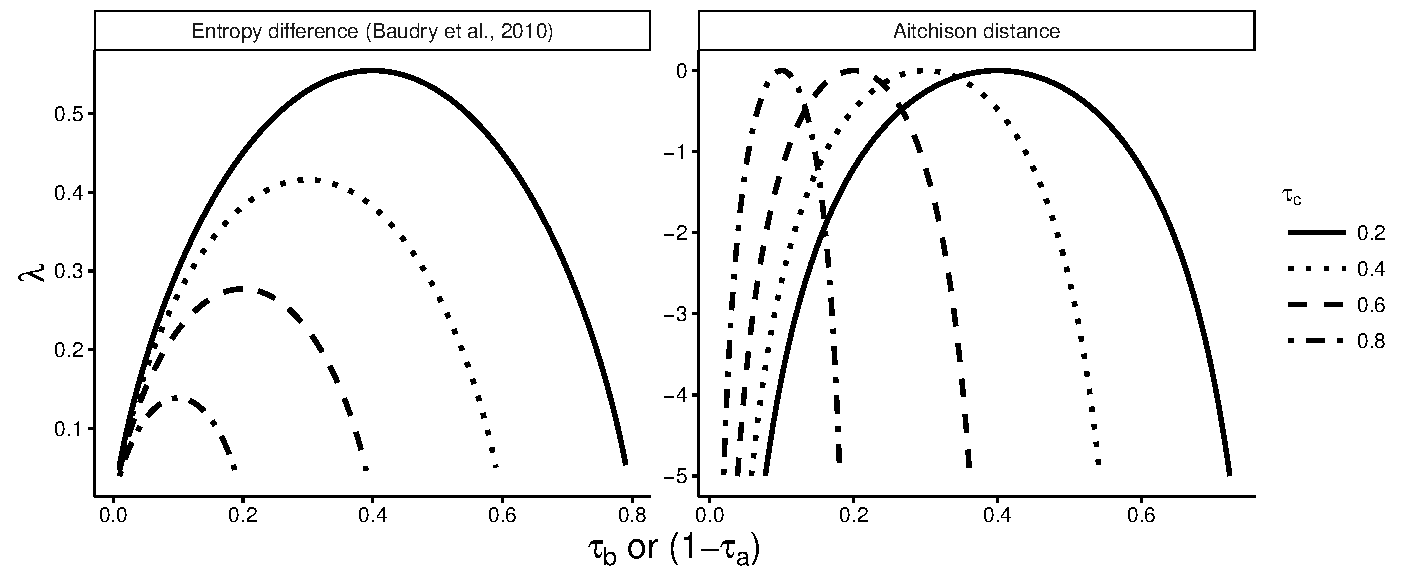
\includegraphics[width=0.8\textwidth]{figures/entr_dist.pdf} \\
 \end{tabular}
 \caption{Comparison between $\lambda_{\Delta\text{Ent}}$ and $\lambda_{\text{dist}}$ function for posterior probability 
vector $\left(\tau_{iI_a}, \tau_{iI_b}, \tau_{iI_c} \right)$ with $\tau_{iI_c} \in \{0.2, 0.35, 0.5, 0.65, 0.8\}$.} 
\label{symetric}
\end{center}
\end{figure}

Similarly to $\lambda_{\Delta\text{Ent}}$ function, $\lambda_{\text{dist}}$ function measures how different is $\m\tau_{\left(I_a, I_b\right)}$ of $\m\tau_2^0$. In Figure~\ref{symetric} the functions for a partition with three, $I_a$, $I_b$, $I_c$ is shown. The different curves are showing the effect of $\tau_{I_b}$ into function $\lambda$ for different values of $\tau_{iI_c}$. We see that both functions have their maximum when $\m\tau_{\left(I_a, I_b\right)} = \m\tau_2^0$, that is when $\tau_{i I_b} = \frac{1-\tau_{i I_c}}{2}$. We see that both functions are symmetric with their maximum. In contrast to function $\lambda_{\Delta\text{Ent}}$, function $\lambda_{\text{dist}}$ measures the similarity between $\m\tau_{\left(I_a, I_b\right)}$ and $\m\tau_2^0$ independently of the value of $\tau_{i I_c}$.

Following \cite{longford2014} a different approach using log-ratios can be defined. We propose to measure the increment of $\tau_{iI_b}$ measuring the relative difference between $\tau_{iI_b}$ an $\tau_{iI_a}$ with the log-ratio
\[
\lambda_{\log}(\m\tau_{i \mathcal{P}_s},  I_a,  I_b) = \log \left(\frac{ \tau_{iI_b} }{ \tau_{iI_a} }\right).
\]

\begin{figure}[t]
\begin{center}
\begin{tabular}{cc}
 %   6 toy mixture
  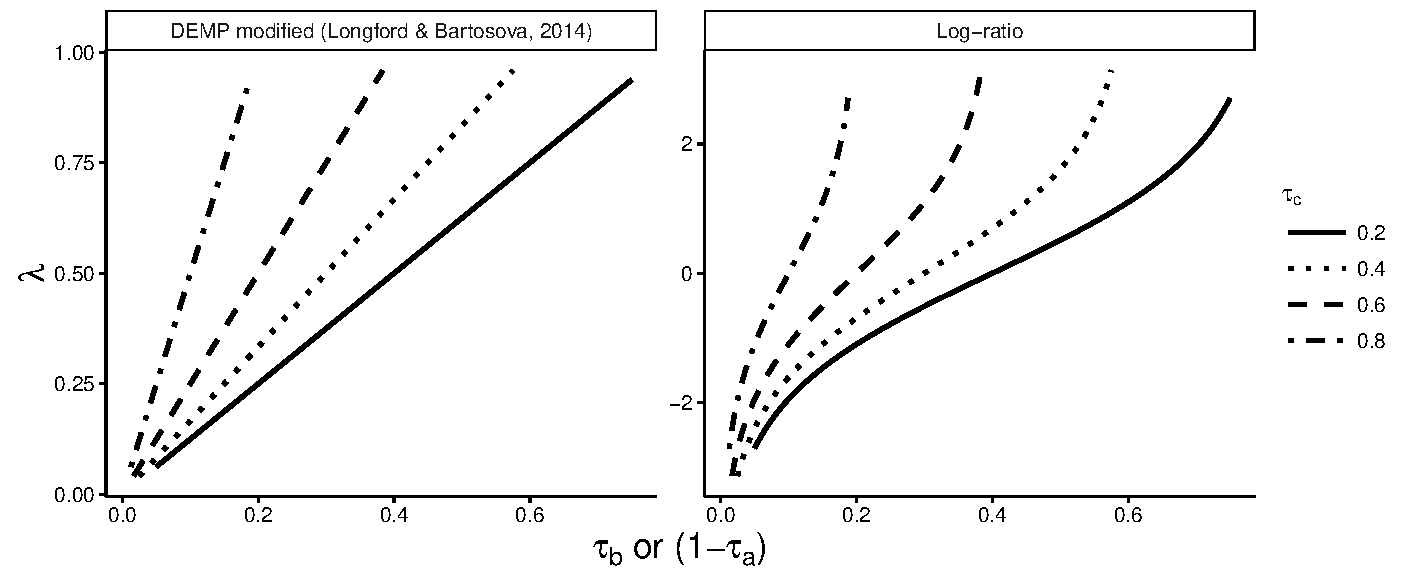
\includegraphics[width=0.8\textwidth]{figures/demp2_log.pdf} \\
 \end{tabular}
 \caption{Comparison between $\lambda_{\text{DEMP}_m}$ and $\lambda_{\log}$ function for posterior probability 
vector $\left(\tau_{iI_a}, \tau_{iI_b}, \tau_{iI_c} \right)$ with $\tau_{iI_c} \in \{0.2, 0.35, 0.5, 0.65, 0.8\}$.} 
\label{nonsymetric}
\end{center}
\end{figure}

In Figure~\ref{nonsymetric} $\lambda_{\text{DEMP}_m}$ and $\lambda_{\log}$ is shown for posterior probability vectors $\left(\tau_{iI_a}, \tau_{iI_b}, \tau_{iI_c}\right)$ for fixed values of $\tau_{iI_c} \in \{0.2, 0.4, 0.6, 0.8\}$. Note that both functions are independent of the value $\tau_{iI_c}$ and only the relative amount between $\tau_{iI_b}$ with respect of $\tau_{iI_a}$ is of importance.

When function $\lambda_{\log}$ is considered we are looking for observations with higher posterior probability $\tau_{iI_b}$ for posterior probability vectors with high $\tau_{iI_a}$, therefore, our preferences are for those observations with highest values of $\tau_{iI_b}$. In this case, it is essential to consider $\omega$ function weighing higher those $\m\tau_{i \mathcal{P}_s}$ with higher values of $\tau_{iI_a}$.

The fact that $\lambda_{\text{dist}}$ and $\lambda_{\log}$ are only measuring the relative difference of $\tau_{iI_a}$ and $\tau_{iI_b}$ makes especially important the selection of function $\omega(\m\tau_{i \mathcal{P}_s},  I_a,  I_b)$. 

It is very important to consider $\omega$ which increase the value of those observation more related with components $f_{I_a}$ or $f_{I_b}$. When we are considering to merge two parts $I_a$ and $I_b$, the ratio for observations that are not representative of this two parts (observations far from been classified into $I_a$ or $I_b$) should be weighted down. Otherwise, the evaluation of $\lambda$ function for those posterior probabilities poorly related to parts $I_a$ and $I_b$ are going to be playing an important role for the final $S$-value. Therefore, this fact makes particularly useless to select function $\omega_{\text{cnst}}$.


Due $\lambda_{\text{dist}}$ and $\lambda_{\log}$ use logratios they take into an account the geometric properties of the Simplex space \citep{aitchison2002simplicial}.  Working with log-ratios between the components of a posterior probability vector, it holds \emph{subcompositional coherence}  \citep{aitchison1986statistical}. This property guarantees that any statistical inference obtained using only partial information is coherent with results obtained using complete information. Formally, in this scenario sub-compositional coherence can be defined as:

\begin{defn}
Let $\mathcal{P}_1, \dots, \mathcal{P}_k$ be a hierarchical sequence of partitions obtained from posterior probability vectors $\text{\textbf{T}}_{\mathcal{P}_k}$ using a merging approach $M$. Let $I = \{j_1, \dots, j_s\}$ be an element of $\mathcal{P}_s$, for some $s$, $1\leq s \leq k$. A method M is \emph{sub-compositional coherent} if the hierarchy subsequence of partitions obtained  using only posterior probability vectors $\left\{ \left(\tau_{ij_1}, \dots, \tau_{ij_s} \right)\right\}_{1\leq i \leq n}$ is contained in original hierarchy.
\end{defn}

Another interesting feature when log-ratio approach is used is the \emph{scale invariance} property, formally
\[
S_{\omega, \lambda}( \m\tau_{\mathcal{P}_s},  I_a,  I_b) = S_{\omega, \lambda}(k\cdot \m\tau_{\mathcal{P}_s},  I_a,  I_b) \text{ for $k>0$.}
\] 

Scale invariance property suggest that the approach is not limited to posterior probability vectors but to any other kind of vector giving relative information between mixture components. In consequence, the methods considered here are suitable to be applied in more general scenarios such that those were instead of posterior probability vectors different weights are given to each part (e.g. weights in fuzzy clustering).




Finally, noting that when $\omega_{\text{prop}}$ and $\lambda_{\log}$ are considered, the $S$-value (Equation~\ref{unifying_equation}) results in
\[
S_{\omega, \lambda}( \m\tau_{\mathcal{P}_s},  I_a,  I_b) = \frac{\sum_{i=1}^n\tau_{iI_a}  \log \left(\frac{ \tau_{iI_b} }{ \tau_{iI_a} }\right)}{\sum_{i=1}^n \tau_{iI_a}}.
\]
For a fixed component $I_a$, the denominator is constant and we only need to maximise the numerator. the expression in the numerator has the flavour of the Kullback-Leibler divergence (in negative sign) comparing the distribution of classifying observations to $I_a$ against the distributions of classifying the same observations to $I_b$.

\section{Deciding the number of clusters}

Given a finite mixture adjusted with BIC criteria, we have presented a generic approach to built a hierarchical sequence of partitions. One of the main difficulties is about deciding the final number of clusters. It is clear that for any partition $\{I_1, \dots, I_{s}\}$ the likelihood function of mixture $\pi_{I_1} f_{I_1} + \dots + \pi_{I_s} f_{I_s}$ is always the same. In other words, it is not possible to decide which of the different relation ways of modelling a cluster with different components is better from a frequentist perspective \citep{hennig2010methods}. Therefore, we need to use heuristic methods to decide the final number of clusters.

\subsection{Using $S$-values}

The first candidates to decide the number of components is to use the $S$-values. In the special case with $\omega_{\text{cnst}}$ and $\lambda_{\Delta\text{Ent}}$ \cite{baudry2010combining} propose to visualise the $S$-values and apply the elbow rule. In the case that $\omega_{\text{prop}}$ and $\lambda_{\text{DEMP}}$ \cite{hennig2010methods} propose to set a threshold and stop merging when the $S$-values is lower that the threshold. It is difficult to define a single method for all methods, but visualising the $S$-values can be a good tool to decide the final number of clusters.

To visualise the $S$-value we can normalise $S$-values to the interval $\left[0,1\right]$. To doing so we have to options, we can either consider only functions $\lambda$ with values in the interval $\left[0,1\right]$ or we can apply a function $g$ to function $S_{\omega, \lambda}$ in such a way that the values of  $g \circ S_{\omega, \lambda}$ are in the interval $\left[0,1\right]$. Because function $S_{\omega, \lambda}$ is a weighed mean function $g \circ S_{\omega, \lambda}$ has the same image as $g \circ \lambda$. In consequence, we need to consider a function $g$ mapping from the domain of $\lambda$ to the interval $\left[0,1\right]$.

From the already introduced functions, $\lambda_{\text{DEMP}}$, $\lambda_{\text{DEMP}_m}$, $\lambda_{\text{prop}}$ and $\lambda_{\text{dist}}$ have domain $\left[0,1\right]$, then their respectively $S_{\omega, \cdot}$ functions are defined in $\left[0,1\right]$ too. Functions $\lambda_{\Delta\text{Entr}}$ and and $\lambda_{\log}$ do not have the image $\left[0,1\right]$, and then, their corresponding $S_{\omega, \cdot}$ functions neither. Possible candidates are $g_{\Delta\text{Entr}}(x) = -x/{\log(\frac{1}{s})}$  and $g_{\log}(x) = \frac{e^x}{1+e^x}$ respectively.

\subsection{Using the clusters of the posterior probabilities}\label{coda_clusters}

\begin{figure}[htbp]
\begin{center}
\begin{tabular}{cc}
 %   6 toy mixture
  \includegraphics[width=0.7\textwidth]{figures/cluster_post.pdf} \\
 \end{tabular}
 \caption{Top-Left: Sample forming three clusters, where each cluster can be modelled by a mixture of two Gaussian distributions. Top-Right: Posterior probability vectors represented in the Simplex space. Because the observations lie close to the border, they are difficult to identify. Bottom-Left: Posterior probability vectors centered and rescaled to have total variance one. Bottom-Right: Posterior probability vectors represented in coordinates with respect an orthonormal basis of the Simplex space.}\label{cluster_post}
\end{center}
\end{figure}

When a sample consists of $s$ well separated clusters, if each cluster is modelled by a different probability distribution, the posterior probability vectors of the elements of one cluster should define a cluster in $\mathcal{S}^s$. For example, in Figure~\ref{cluster_post} we have a sample with three different clusters. The observations are modelled by a Gaussian mixture with six components (top-left). After merging the components into three components, each one formed with a mixture of two components, the posterior probability vectors are elements of $\mathcal{S}^3$. Although the observations have some component very close to zero, we can represent the posterior probability vectors in a ternary diagram (top-right). To better visualise the posterior probability we can center and scale the posterior probability vectors (bottom-left). Note that the relative Aitchison distance between posterior probability vectors before and after centering is conserved. For better visualise the structure of posterior probability vectors we can express each one with respect a orthonormal basis of $\mathcal{S}^3$ (bottom-right). Note that the posterior probability are also forming three different clusters.


Therefore, another approach to decide the number of components using the posterior probability vectors $\text{\textbf{T}}_{\mathcal{P}_s}$ is to consider each posterior probability vector $\m\tau_{i\mathcal{P}_s}$ as an element of $\mathcal{S}_s$. Then, we can work with the geometric structure of $\mathcal{S}_s$ to study the relation between different posterior probability vectors. Concretely, using the Aitchison distance, we can compute the distance between each pair of posterior probability vectors. With this matrix distance we can study how well the components $f_{I_1}, \dots, f_{I_s}$ are defining the clusters. We expect that those posterior probabilities more related to one cluster are close to the vertex of the Simplex space, i.e. have values close to one in one component and close to zero in the other components. Consequently, we expect that the posterior probabilities vectors in $\mathcal{S}_s$ define $s$ different clusters.

A last option is not stopping the hierarchical merging and presenting the overall sequence of partitions. This approach should allow the researcher to study carefully how the initial components are related to each other in each step.


\section{Merging components in a finite mixture: examples}\label{merging_examples_dist}

\subsection{Merging components in a mixture of Gaussian distributions}

Following the example given in \cite{baudry2010combining} consider the bivariate Gaussian mixture of six components
\[
f= \sum_{j=1}^6 \pi_j \phi(\;\cdot\; ;  \m\mu_j, \m\Sigma_j)
\]
with parameters shown at Table~\ref{pars_table}. 

\begin{table}[t]
\centering
\begin{tabular}{rrrrrrr}
  \hline
$j$ & $\pi_j$ & $\mu_{j x_1}$ & $\mu_{j x_2}$ & $\sigma^2_{j x_1}$ & $\sigma^2_{j x_2}$ & $\rho_{j x_1 x_2}$ \\ 
  \hline
  1 &  $1/6$ &     0 &     0 &    50 &     5 &     0 \\ 
  2 &  $1/6$  &     0 &    40 &     5 &    50 &     0 \\ 
  3 &  $1/6$  &    40 &    40 &     5 &    50 &     0 \\ 
  4 &  $1/6$  &     0 &     0 &     5 &    50 &     0 \\ 
  5 &  $1/6$  &    40 &     0 &    50 &     5 &     0 \\ 
  6 &  $1/6$  &    40 &    40 &    50 &     5 &     0 \\ 
   \hline
\end{tabular}
\caption{Parameters defining a two dimensional Gaussian mixture with six components. The parameters $\m\mu_j$ and $\m\Sigma_j$ are expressed in terms of the univariate means $\mu_{j x_1}$, $\mu_{j x_2}$, the univariate variances $\sigma^2_{j x_1}$, $\sigma^2_{j x_2}$ and the correlation between $x_1$ and $x_2$, $\rho_{j x_1 x_2}$.}
\label{pars_table}
\end{table}


Let the parameters of $f$ be known. Figure~\ref{ex_mixture} shows a random sample \textbf{X} together with the isodensity curves of the estimated \fmm. We are interested in clustering the sample \textbf{X}.

\begin{figure}[htbp]
\begin{center}
\begin{tabular}{cc}
 %   6 toy mixture
  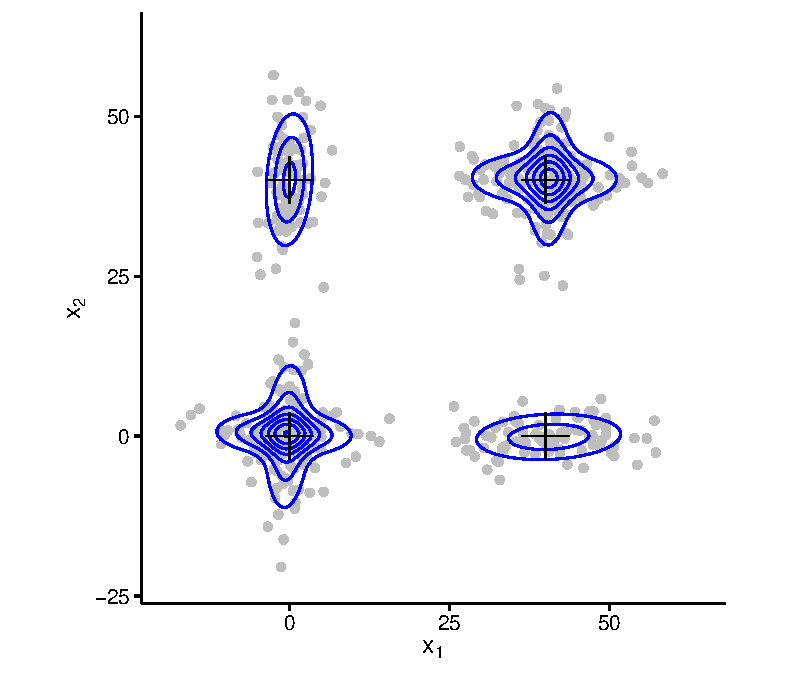
\includegraphics[width=0.7\textwidth]{figures/partition-example-mixture.pdf} \\
 \end{tabular}
 \caption{Density of Gaussian mixture of 6 components. Sample mean estimated of each component is represented by '+'.}\label{ex_mixture}
\end{center}
\end{figure}

The initial partition  $\mathcal{P}_6 = \{ \{1\},\{2\}, \{3\}, \{4\}, \{5\}, \{6\} \}$  by Equation~\ref{cluster_criteria} yields to a six clusters were each component is associated to one cluster. In Figure~\ref{ex_one_one} we have separate the observations in its respective cluster. In the plot we show isodensity curves for the density modelling each cluster. In this case each cluster is modelled with a Gaussian distribution.

\begin{figure}[h]
\begin{center}
\begin{tabular}{cc}
 %   6 toy mixture
  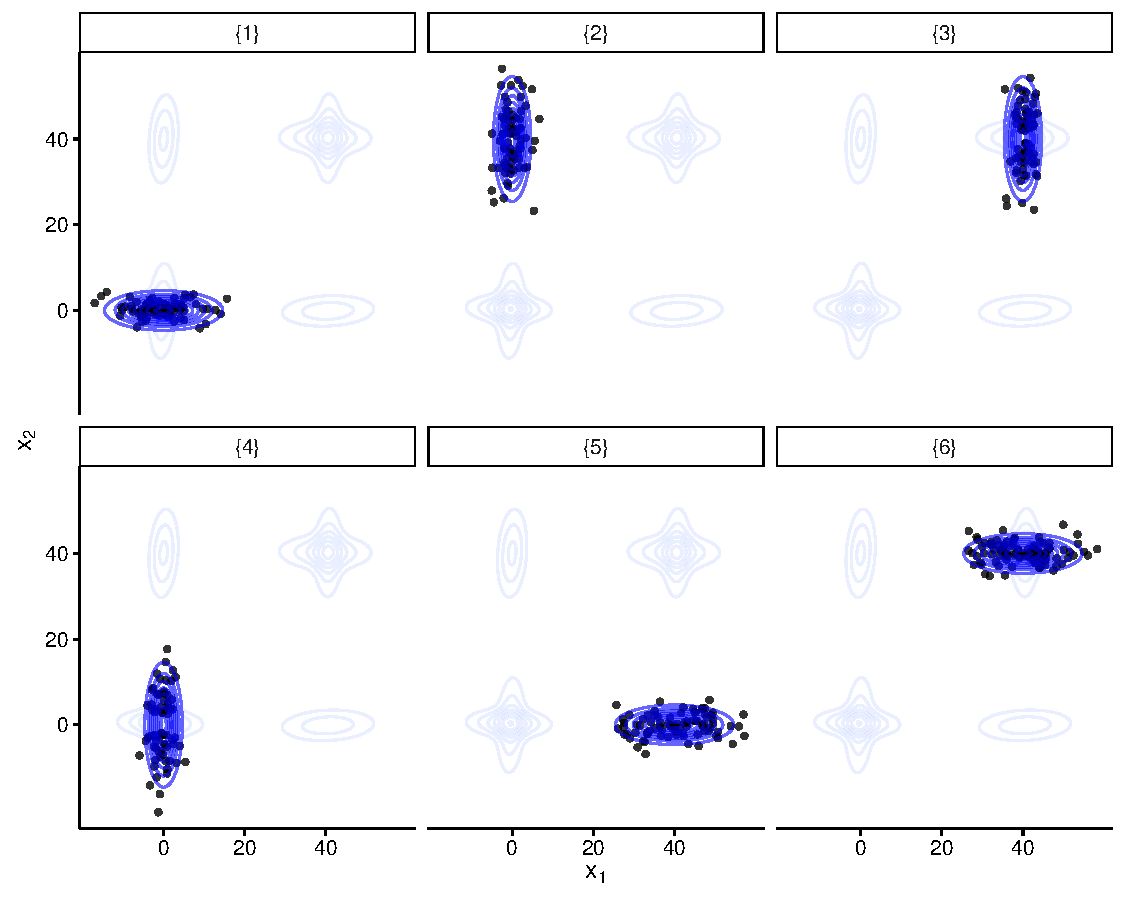
\includegraphics[width=\textwidth]{figures/partition-example-part6.pdf} \\
 \end{tabular}
 \caption{Density of Gaussian mixture of 6 components where one cluster corresponds to one component}\label{ex_one_one}
\end{center}
\end{figure}

With the posterior probabilities $\text{\textbf{T}}_{\mathcal{P}_s}$ we calculate the $S$-values with $\omega_{\text{cnst}}$ and $\lambda_{\Delta\text{Ent}}$. We obtained the sequential hierarchical partition given by 

\begin{equation}
\begin{array}{r c l}
\mathcal{P}_1 &=& \{\{1, 2, 3, 4, 5, 6\}\}, \\
\mathcal{P}_2 &=& \{\{1, 2 , 4, 5\}, \{3, 6\} \},  \\
\mathcal{P}_3 &=& \{\{1, 2, 4\}, \{3, 6\}, \{5\} \}, \\
\mathcal{P}_4 &=& \{\{1, 4\},\{2\}, \{3, 6\}, \{5\} \}, \\
\mathcal{P}_5 &=& \{\{1\},\{2\}, \{3, 6\},\{4\},\{5\} \},\\
\mathcal{P}_6 &=& \{\{1\},\{2\},\{3\},\{4\},\{5\},\{6\}\}.
\end{array}
\label{hier_ex}
\end{equation}

In the partition $\mathcal{P}_4 = \{\{1, 4\},\{2\}, \{3, 6\}, \{5\} \}$, the part $\{1, 4\}$ define a single cluster, as well as part \{3, 6\}. For this partition, using Equation~\ref{cluster_criteria} each observation $\m x_i$ is classified to one component. Figure~\ref{ex_two_one} shows the clustering with the isodensity curves defined by each component. In this case, clusters labelled $\{1,4\}$ and $\{3, 6\}$ are modelled by a mixture of two components. With partition $\mathcal{P}_4$ the clusters are modelled by $\fmm$s
\begin{itemize}
\item $f_{\{1,4\}} = \frac{1}{2} \phi(\;\cdot\; ;  \m\mu_1, \m\Sigma_1) + \frac{1}{2} \phi(\;\cdot\; ;  \m\mu_4, \m\Sigma_4)$, 
\item $f_{\{2\}} = \phi(\;\cdot\; ;  \m\mu_2, \m\Sigma_2)$, 
\item $f_{\{3,6\}} =  \frac{1}{2} \phi(\;\cdot\; ;  \m\mu_3, \m\Sigma_3) + \frac{1}{2} \phi(\;\cdot\; ;  \m\mu_6, \m\Sigma_6)$ and
\item $f_{\{5\}} = \phi(\;\cdot\; ;  \m\mu_5, \m\Sigma_5)$.
\end{itemize}

\begin{figure}[h]
\begin{center}
\begin{tabular}{cc}
 %   6 toy mixture
  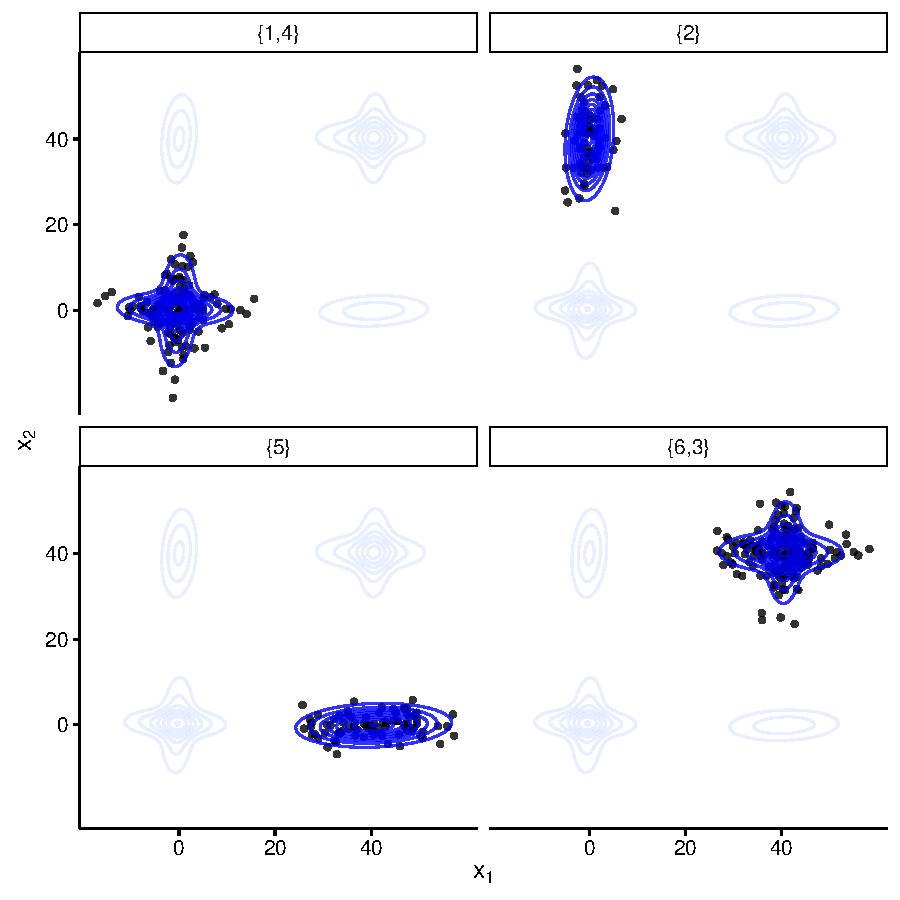
\includegraphics[width=0.65\textwidth]{figures/partition-example-part4.pdf} \\
 \end{tabular}
 \caption{Density of Gaussian mixture of 6 components where one cluster corresponds to one or more components}\label{ex_two_one}
\end{center}
\end{figure}

With $\omega_{prop}$ combined with $\lambda_{\text{DEMP}_m}$, $\lambda_{\text{dist}}$, $\lambda_{\log}$ and $\lambda_{\text{prop}}$ we obtain the same hierarchical partition \ref{hier_ex}. Using $\omega_{prop}$ and $\lambda_{\text{DEMP}}$ the sequential hierarchical obtained only differs from the previous one  in partition $\mathcal{P}_5$, where now $\mathcal{P}_5 = \{\{1, 4\},\{2\}, \{3\},\{5\},\{6\} \}$.

To decide the number of clusters in Figure~\ref{gaussian_Svalues} we plot the $S$-values using different approaches (upper plot) and using the Aitchison distance between posterior probabilities we calculate the Calinski-Harabasz (G1) and the Goodman and Kruskal (G2) indices \citep{milligan1985}. We also include the average between and within clusters to monitor the process. (lower plot). Except the log-ratio approach before scaling, we see that all approaches after merging components to model four clusters or less the $S$-values are close to zero. This indicates that the clustering defined with four, three, or two clusters are well separated. Both G1 and G2 have a local maximum in four clusters, indicating that by those methods it is preferred to separate the data into four clusters. Combining the information obtained with the $S$-values and the indices G1 and G2 we separate our data into four clusters using partition $\mathcal{P}_4$ as shown in Figure~\ref{ex_two_one}.

\begin{figure}[t]
\begin{center}
\begin{tabular}{cc}
  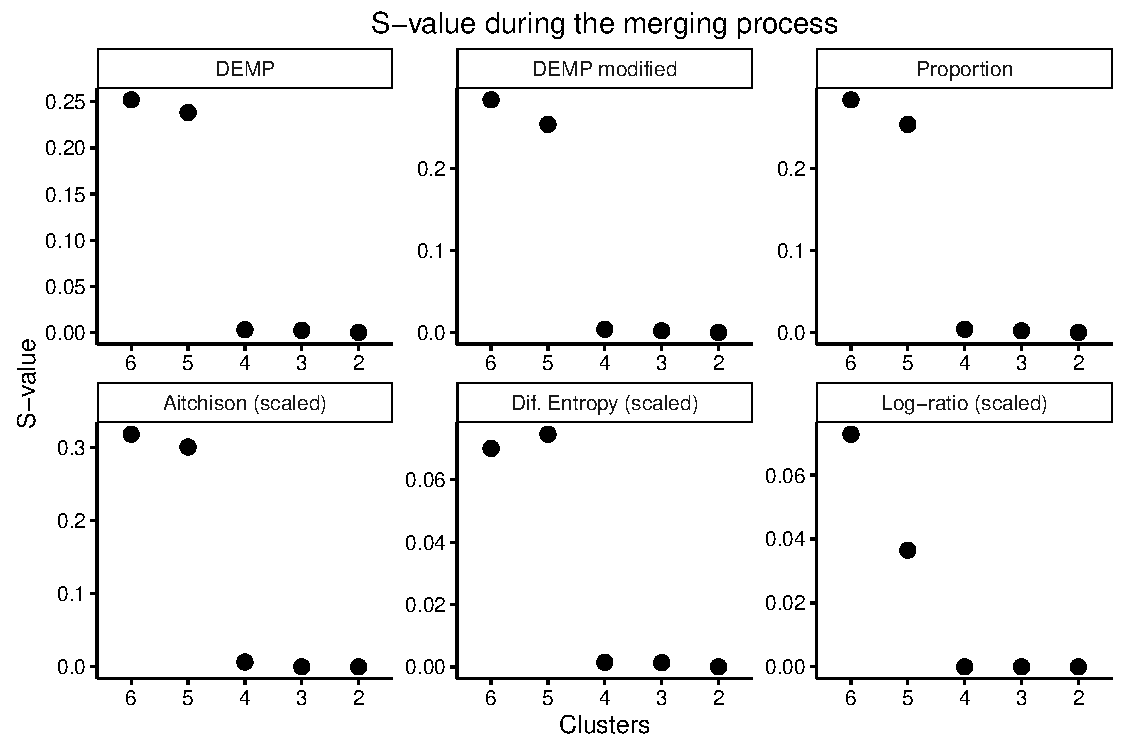
\includegraphics[width=0.85\textwidth]{figures/gaussian_Svalues.pdf} \\
   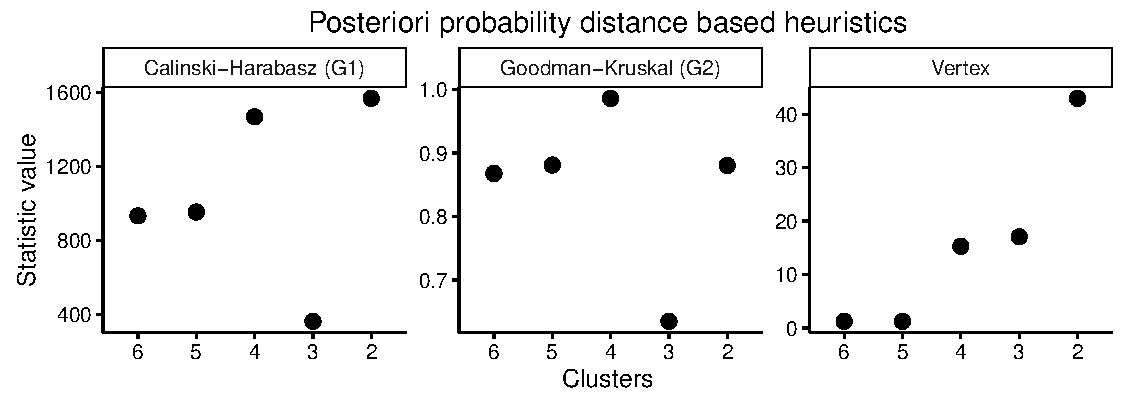
\includegraphics[width=0.85\textwidth]{figures/gaussian_statistics.pdf}
 \end{tabular}
 \caption{S-values obtained using the approaches presented by Baudry et al. and Hennig labeled Entropy and DEMP respectively.}\label{gaussian_Svalues}
\end{center}
\end{figure}

\subsection{Merging components in a mixture of multinomial distributions}\label{multinom_example}

Merging approaches presented in this article rely on the vector of posterior probabilities which can be calculated for any finite mixture model. Therefore, the merging generic approach introduced in Section~\ref{generic_merging} can be used for any family of \fmm, for example a finite mixture of multinomial distribution.

Pigs dataset can be obtained from package \emph{zCompositions} R package \citep{palarea2015zcompositions}. The dataset contains data of 29 sows. In different moments the pigs were recorded during five minutes and its current activity was registered. For each pig six locations were considered: straw bed (BED), half in the straw bed (HALF.BED), dunging passage (PASSAGE), half in the dunging passage (HALF.PASS), feeder (FEEDER) and half in the feeder (HALF.FEED).


\begin{table}[t]
\centering
\begin{tabular}{rrrrrrrr}
  \hline
 Comp.& $\pi_j$ & $\theta_{j1}$ & $\theta_{j2}$ & $\theta_{j3}$ & $\theta_{j4}$ & $\theta_{j5}$ & $\theta_{j6}$ \\ 
  \hline
  1 & 0.0695 & 0.0103 & 0.0000 & 0.2874 & 0.0103 & 0.6867 & 0.0052 \\ 
  2 & 0.1710 & 0.0144 & 0.0000 & 0.0717 & 0.0020 & 0.9057 & 0.0062 \\ 
  3 & 0.0699 & 0.0817 & 0.0102 & 0.1390 & 0.0000 & 0.7538 & 0.0154 \\ 
  4 & 0.1724 & 0.1567 & 0.0082 & 0.7835 & 0.0021 & 0.0454 & 0.0041 \\ 
  5 & 0.0345 & 0.9485 & 0.0000 & 0.0309 & 0.0000 & 0.0206 & 0.0000 \\ 
  6 & 0.4828 & 0.7408 & 0.0147 & 0.1694 & 0.0074 & 0.0626 & 0.0052 \\  
   \hline
\end{tabular}
\caption{Parameters of a finite mixture of multinomial distributions adjusted to the Pigs data set. For component $j$, the mixing proportions are denoted by $\pi_j$ and the multinomial probabilities by $\left(\theta_{j1}, \dots, \theta_{j6}\right)$.}\label{multinomial_pars}
\end{table}

We used \emph{mixtools} \citep{benaglia2009mixtools} to fit a multinomial mixture. Six components were identified as optimum according to BIC criterion. In Table~\ref{multinomial_pars} the parameters of each components are shown. Using this parameters we can compute the posterior probability vectors $\text{\textbf{T}}_{\mathcal{P}_6}$. Each observation is classified into one cluster following Equation~\ref{map_criteria} or Equation~\ref{cluster_criteria} with partition $\mathcal{P}_6 = \{\{1\}, \{2\}, \{3\}, \{4\}, \{5\}, \{6\}\}$. In Figure~\ref{multinomial_mixture} we can see the bar plot for observations classified into the same cluster.

\begin{figure}[!t]
\begin{center}
\begin{tabular}{cc}
  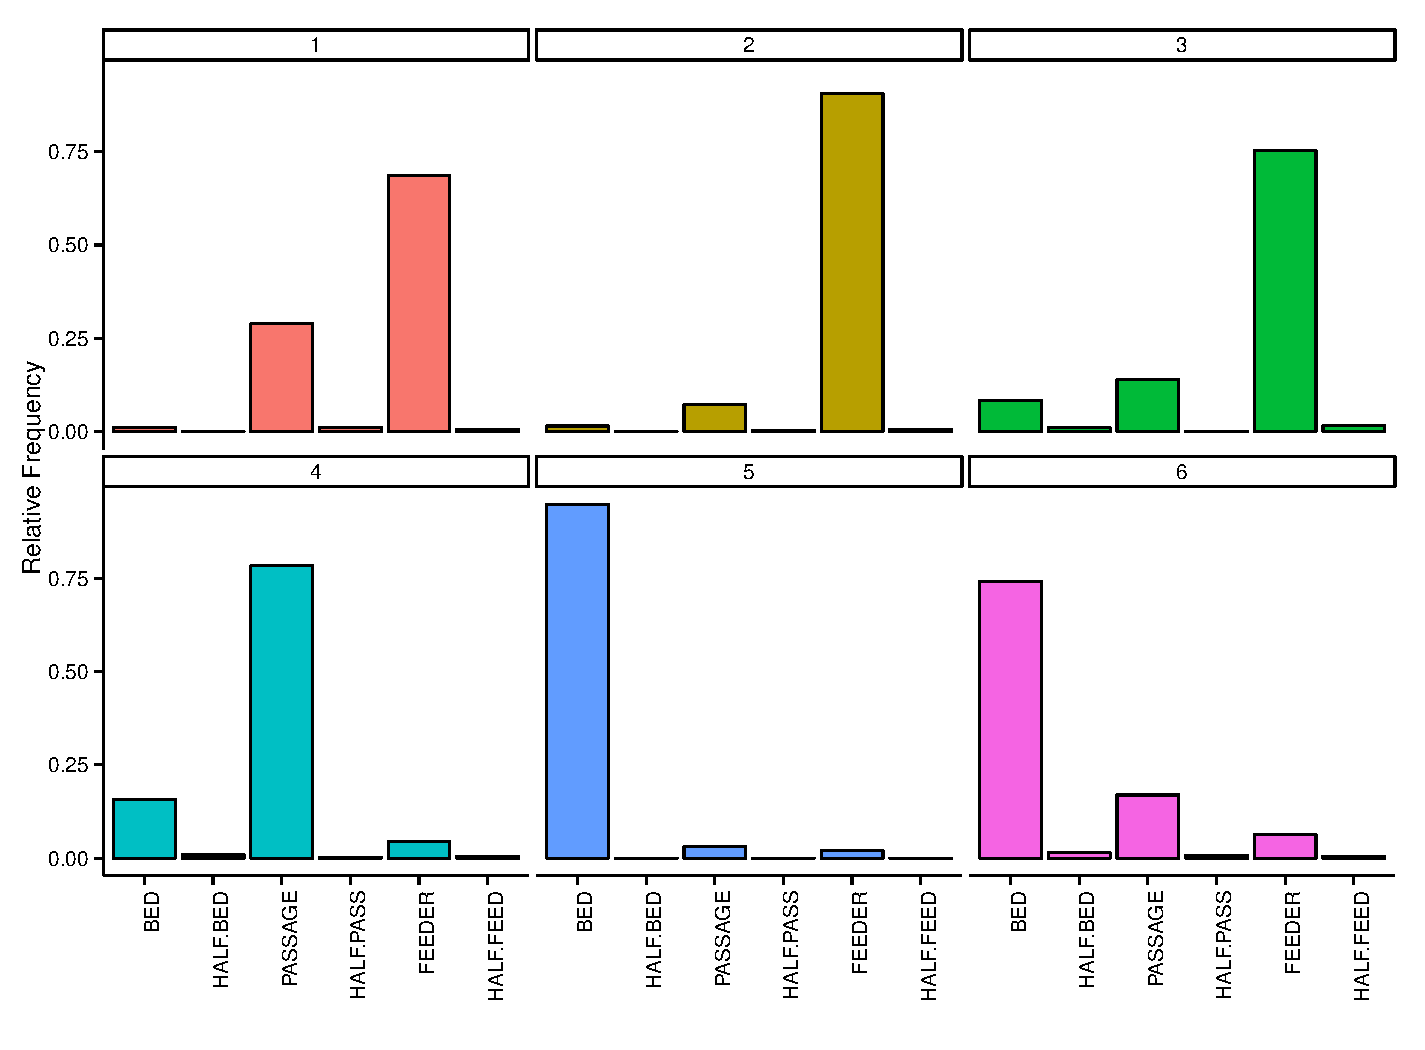
\includegraphics[width=0.95\textwidth]{figures/multinomial_mixt_all.pdf} \\
 \end{tabular}
 \caption{Components after adjusting a six mixture of multinomial distributions. For each cluster, the relative amount of time seen in each location is shown.}\label{multinomial_mixture}
\end{center}
\end{figure}

Using $\omega_{\text{dich}}$ or  $\omega_{\text{prop}}$ with $\lambda_{\text{dist}}$ or $\lambda_{\log}$ we obtained the hierarchical structure partition given by


\begin{equation}
\begin{array}{r c l}
 \mathcal{P}_1&=& \{\{1,2,3,4,5,6\}\}, \\ 
 \mathcal{P}_2&=& \;\; \{\{1,2,3\},\{4,5,6\}\}, \\ 
 \mathcal{P}_3&=& \;\; \{\{1,2,3\},\{4\},\{5,6\}\}, \\ 
 \mathcal{P}_4&=& \;\; \{\{1,2\},\{3\},\{4\},\{5,6\}\}, \\ 
 \mathcal{P}_5&=& \;\; \{\{1\},\{2\},\{3\},\{4\},\{5,6\}\}, \\ 
 \mathcal{P}_6&=& \;\; \{\{1\},\{2\},\{3\},\{4\},\{5\},\{6\}\}.
\end{array}
\label{hier_ex_multinomial}
\end{equation}

Other methods like $\omega_{\text{csnt}}$-$\lambda_{\Delta\text{Ent}}$,  $\omega_{\text{prop}}$-$\lambda_{\text{DEMP}}$,  $\omega_{\text{prop}}$-$\lambda_{\text{prop}}$ differed only in partitions $\mathcal{P}_5$ and $\mathcal{P}_4$.  Instead, this methods preferred to merge first the part $\{1,2,3\}$ obtaining partitions $\mathcal{P}_5 = \{\{1\},\{2, 3\},\{4\},\{5\} ,\{6\}\}$ and $\mathcal{P}_4 = \{\{1,2,3\},\{4\},\{5\},\{6\}\}$.

\begin{figure}[th]
\begin{center}
\begin{tabular}{cc}
  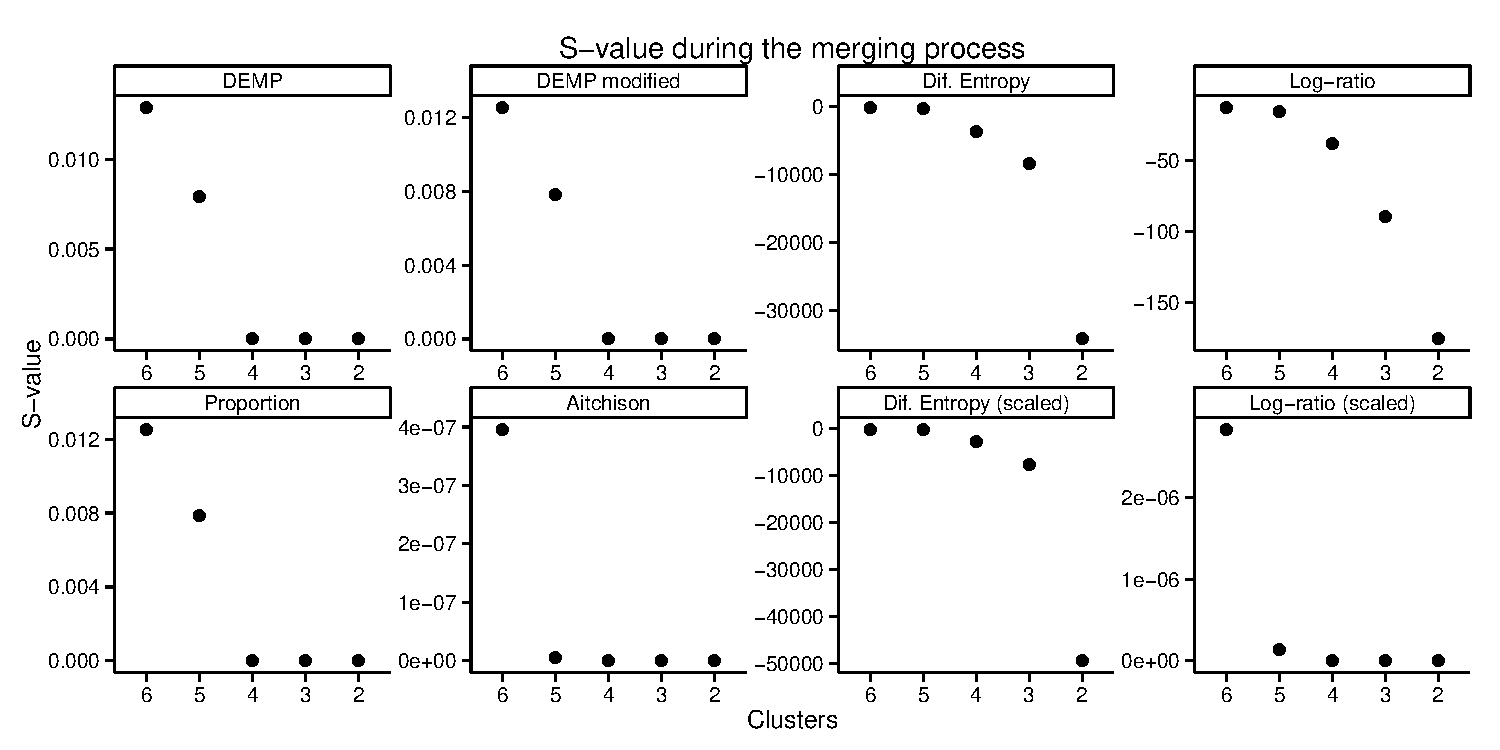
\includegraphics[width=0.85\textwidth]{figures/multinomial_Svalues_all.pdf} \\
  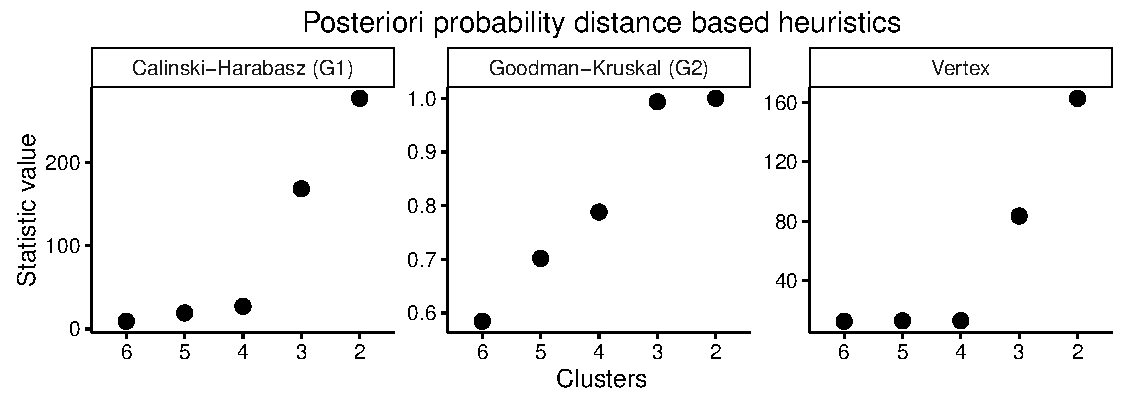
\includegraphics[width=0.85\textwidth]{figures/multinomial_statistics.pdf} \\
  \includegraphics[width=0.85\textwidth]{figures/multinomial_statistics2.pdf} 
 \end{tabular}
 \caption{Squared average distance between clusters (top-left), the squared average distance within clusters (top-right), the Calinski-Harabasz index (bottom-left) and the Goodman and Kruskal's Gamma coefficient (bottom-right) applied to the posterior probabilities obtained after adjusting a finite mixture of multinomial distributions to the Pigs data set.}\label{multinomial_statistics}
\end{center}
\end{figure}

\begin{figure}[t]
\begin{center}
\begin{tabular}{cc}
  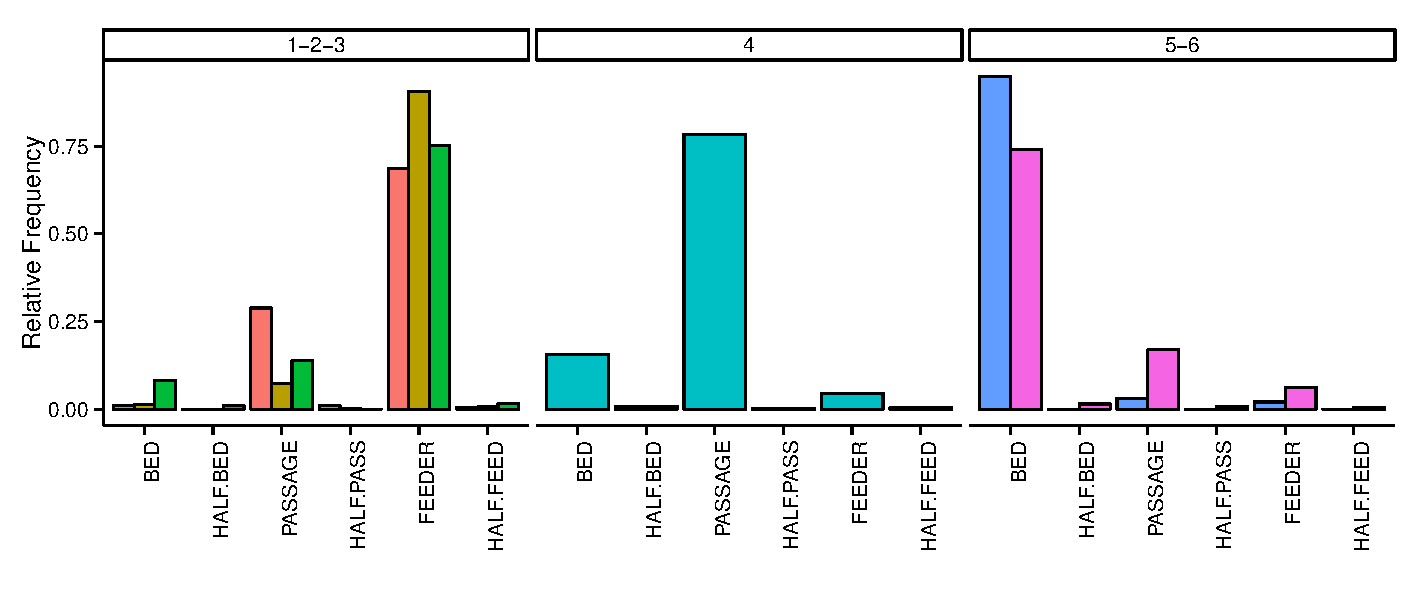
\includegraphics[width=0.95\textwidth]{figures/multinomial_clust3_all.pdf} \\
 \end{tabular}
 \caption{Pig dataset components after clustering the six mixture components in a 3-\fmm. For each cluster, the relative amount of time seen in each location is shown.}\label{multinomial_clust3}
\end{center}
\end{figure}

In Figure~\ref{multinomial_statistics} we plot the $S$-values given by different approaches (upper plot). We also plot the between and within averaged squared distances and the G1 and G2 index (lower plot). Except for the log-ratio approach (before and after scaling) and the squared distance, the $S$-values are close to zero after merging the components into four clusters. The squared distance and the log-ratio approach have an $S$-value close to zero after merging the components into five clusters. Depending on the method, we can see that when the clustering is modelled by five (four) clusters or less, the clusters are well separated. Inspecting the plot with the G1 and G2 indices, it indicates that the best choice is two clusters for $G1$ and three clusters for $G2$. Figure~\ref{multinomial_clust3} shows the bar plot for those observations assigned to each of the three clusters. The first cluster contains components one, two and four, all of them represented by sows with a high amount of time feeding. The second cluster contains components three and five, this cluster is characterized by sows with high amount of time in bed. Finally, the third cluster is form with a single component six which have a higher amount of time in the passage.



\section{Final remarks}\label{remarks}

When \fmm is used in clustering the question \textit{``is a cluster determined by a unique component?''} emerges. Different authors have proposed scenarios where it seems reasonable to argue that a cluster can be better modelled by more than one single component, or equivalently, modelled by a \fmm itself. In this scenarios, the approaches proposed in this article can be of interest.

In literature different approaches have been considered to merge the components of a \fmm. Some of them are specific to a particular type of mixture (methods related to Gaussian mixtures) and some others are independent of the type of mixture (to cite generic approaches). The generic approach proposed in this articles relies only on the posterior probability vectors, and therefore, it is independent from the family of mixture. All the methods described in this article can be applied with any \fmm. We have illustrated the approach with a numerical sample and with categorical sample. 

The log-ratio approaches introduced in this article (Section~\ref{logratio_section}) and the indices defined on the posterior probabilities (Section~\ref{coda_clusters}) use the geometric structure of the Simplex space. Working with the posterior probabilities as an elements of the Simplex space permits to extend the results obtained here in other areas. For example, it would be interesting to analyse if in fuzzy-clustering the role played by the weights is equivalent to the role played by the posterior probabilities. 

Finally, to decide final number of clusters we have proposed to combine the information given by the $S$-values and to analyse some heuristic like the Calinski-Harabasz index or  the Goodman and Kruskal index. To the best of our knowledge it is the first time that has been proposed to study the cluster structure using distance based heuristics on the posterior probability vectors. This new approach allows to study the structure of numerical and categorical data sets based on the considered model.


%%% BIBLIOGRAPHY

%\bibliographystyle{apalike}
\begin{thebibliography}{}

\bibitem[Aitchison, 1986]{aitchison1986statistical}
Aitchison, J. (1986).
\newblock {\em {The Statistical Analysis of Compositional Data}}.
\newblock Monographs on Statistics and Applied Probability. Chapman \& Hall Ltd., London (UK). Reprinted (2003) with additional material by The Blackburn Press, Caldwell, NJ.

\bibitem[Aitchison, 2002]{aitchison2002simplicial}
Aitchison, J. (2002).
\newblock {\em {Simplicial inference}}.
\newblock {\em Algebraic Methods in Statistics anb Probability}, 287: 1--22.

\bibitem[Baudry et~al., 2010]{baudry2010combining}
Baudry, J.P., Raftery, A.~E., Celeux, G., Lo, K., and Gottardo, R. (2010).
\newblock {Combining Mixture Components for Clustering}.

\bibitem[Benaglia et~al., 2009]{benaglia2009mixtools}
Benaglia, T., Chauveau, D., Hunter, D.R. and Youn, R. (2009).
\newblock {mixtools: An R Package for Analyzing Finite Mixture Models}.
\newblock {\em Journal of Statistical Software}, 32(6), 1--29.

\bibitem[Fraley and Raftery, 1998]{fraley1998how}
Fraley, C. and Raftery, A. E. (1998).
\newblock {How many clusters? Answers via model-based cluster analysis}.
\newblock {\em The computer Journal}, 41:578--588.

\bibitem[Fraley and Raftery, 2002]{fraley2002model}
Fraley, C. and Raftery, A. E. (2002).
\newblock {Model-Based Clustering, Discriminant Analysis, and Density Estimation}.
\newblock {\em Journal of the American Statistical Association}, 97(458):611--631.

\bibitem[Hennig, 2010]{hennig2010methods}
Hennig, C. (2010).
\newblock {Methods for merging Gaussian mixture components}.
\newblock {\em Advances in Data Analysis and Classification}, 4(1):3--34.

\bibitem[Keribin, 1998]{keribin1998consistent}
Keribin, C. (1998).
\newblock {Consistent estimate of the order of mixture models}.
\newblock {\em Comptes Rendues de l’Academie des Sciences, Série I-Mathématiques}, 326:243--248.

\bibitem[Keribin, 2000]{keribin2000consistent}
Keribin, C. (2000).
\newblock {Consistent Estimation of the Order of Mixture Models}.
\newblock {\em Sankhy\={a}: The Indian Journal of Statistics, Series A}, 62(1):49--66.

\bibitem[Lee and Cho, 2004]{lee2004combining}
Lee, H.J. and Cho, S. (2004).
\newblock {Combining Gaussian Mixture Models}.
\newblock In Yang, Z., Yin, H., and Everson, R., editors, {\em Intelligent Data
  Engineering and Automated Learning – IDEAL 2004 SE - 98}, volume 3177 of
  {\em Lecture Notes in Computer Science}, pages 666--671. Springer Berlin
  Heidelberg.

\bibitem[Longford and Bartosova, 2014]{longford2014}
Longford, N.~T. and Bartosova, J. (2014).
\newblock {A confusion index for measuring separation and clustering}.
\newblock {\em Statistical Modelling}, 14(3):229--255.

\bibitem[McLachlan, 2014]{mclachlan2014components}
McLachlan, G. J. and Rathnayake S. (2014).
\newblock {On the number of components in a Gaussian mixture model}.
\newblock {\em Wiley Interdisciplinary Reviews: Data Mining and Knowledge Discovery},  4:341--355.

\bibitem[Melnykov, 2013]{melnykov2013distribution}
Melnykov, V. (2013).
\newblock {On the Distribution of Posterior Probabilities in Finite Mixture Models with Application in Clustering}.
\newblock {\em Journal of Multivariate Analysis}, 122:175--189.

\bibitem[Milligan, 1985]{milligan1985}
Milligan, G. W. and Cooper, M. C. (1985) 
\newblock {An examination of procedures for determining the number of clusters}. 
\newblock {\em Psychometrika}, 50:159-179.

\bibitem[Palarea-Albaladejo et~al., 2012]{palarea2012dealing}
Palarea-Albaladejo, J., Martín-Fernández, J.A. and Soto, J.A. (2012).
\newblock {Dealing with Distances and Transformations for Fuzzy C-Means Clustering of Compositional Data}.
\newblock {Journal of Classification}, 29(2):144--169.


\bibitem[Palarea-Albaladejo and Martín-Fernández (2015)]{palarea2015zcompositions}
Palarea-Albaladejo J. and Martin-Fernandez J.A. (2015).
\newblock {zCompositions - R packages for multivariate imputation of nondetecteds and zeros in compositional data sets}.
\newblock{\em Chemometrics and Intelligent Laboratory Systems}, 143:85--96.

\bibitem[Pastore and Tonellato, 2013]{pastore2013merging}
Pastore, A. and Tonellato, S.~F. (2013).
\newblock {A Merging Algorithm for Gaussian Mixture Components}.
\newblock {\em SSRN Electronic Journal}, (04).

\bibitem[Punzo, 2014]{punzo2014flexible}
Punzo, A. (2009).
\newblock {Flexible mixture modelling with the polynomial Gaussian cluster-weighted model}.
\newblock {\em Statistical Modelling}, 14(3):257--291.

\end{thebibliography}

%%%%%%%%%%% END SPACING
%\end{spacing}

\end{document}
